\documentclass[12pt]{article}% 这是主要的格式。
\usepackage[UTF8]{ctex}
\usepackage[page,title,titletoc,header]{appendix} 
\usepackage{enumerate}
\usepackage{amsmath}
\usepackage{graphicx}
\usepackage[labelsep=space]{caption}
\usepackage{cite}
\usepackage{amsthm}
\usepackage{textcomp}
\usepackage{longtable}
\usepackage{array}
\usepackage{bigstrut}
\usepackage{geometry}
\usepackage{gensymb}
\usepackage{graphicx}  
\usepackage{subcaption}
\usepackage{xcolor}  
\usepackage{listings}  
\usepackage{color}  
\geometry{left =2.5 cm,right=2.5cm,top=2.5cm,bottom=2.5cm}
\usepackage[section]{placeins}
\usepackage[colorlinks,linkcolor=black,citecolor=black]{hyperref}
\usepackage{titlesec}  
\usepackage{titletoc}
\setcounter{section}{-1}
\titleformat{\subsection}{\heiti \fontsize{13pt}{0}}{\bf\thesubsection}{0.3em}{}
\titleformat{\subsubsection}{\heiti \fontsize{13pt}{0}}{\thesubsubsection}{0.3em}{}
\renewcommand\figurename{\heiti\zihao{5} 图}
\renewcommand\tablename{\heiti\zihao{5} 表}

\title{ \heiti\zihao{3}裂相(分相)电路的设计与仿真研究}
\author{9161040G0734 许晓明}
\date{}

\begin{document}
%\hypersetup{CJKbookmarks=true}
\maketitle
\abstract{裂相(分相)电路是一种将单相电源分裂成二相或二相以上的电源的电路。在获得旋转磁场、增加整流滤波效果、获取三相电源等方面有着一定的应用。\par
本文通过RC桥式电路,借助multisim仿真软件,探究裂相电路的形成条件以及裂相电路下,各负载与其两端电压、功率之间的数值、趋势关系,来研究裂相电路的相关特性。\par
通过相量图原理分析,本文给出了用单相电源分相成二相、三相电源的一种电路及参数设置方案,并给出具体的参数值。借助对多种负载情况下的电压及功率情况的测量,得到电压、功率与负载间的特性关系,并给出部分裂相电源的具体用途。
\noindent{\\\ \\
\textbf{关键词:} multisim仿真\ 裂相电路\ 电压-负载特性\ 负载功耗 }
}

\titleformat{\section}{\centering\heiti\zihao{4}}{\thesection}{0.3em}{}
\tableofcontents
\titleformat{\section}{\heiti\zihao{4}}{\bf\thesection}{0.3em}{}
\newpage
 \fontsize{12.5pt}{0}
\section{引言}
\subsection{问题的背景}
裂相(分相)电路是一种将单相电源分裂成二相或二相以上的电源的电路。在获得旋转磁场、增加整流滤波效果等方面有着一定的应用。尤其是在获得三相电源方面,常见的三相正弦交流电是由三相交流发电机
产生的,但在有些场合许多民用及教学演示等场合,往往没有三相电源。裂相电路在一定条件下可以在单相电源的作用下获得对称的三相电源,从而,使仅有单相电源供电的场合,能够运用需要三相电源的设备。

那么,如何将单相电源裂相成具有特定相位差的多相电源,以及在裂相电路中,各种情况的负载与其电压、功率的关系就成了需要研究的内容。
\subsection{文献综述}
张继和,刘宗等在裂相电路的研究中推导出了裂相电路总电流与负载电流之间的关系、裂相电路总功率因数与负载功率因数的关系\cite{1},也推导出了强感性和强容性负载所对应的裂相电路\cite{3};刘正生,夏敦柱等则从L -C裂相电路出发 ,深入研究了三相对称负载性质、参数与裂相电路结构、参数之间的关系\cite{2};林道同则相应的研究中提供了两种比较简单、可输出一定功率的裂相电路\cite{4}。\par

参考以上文献并结合课本和相关所学知识,借助multisim仿真进行裂相实验。
\subsection{需要解决的问题}
\begin{enumerate}[1)]
\item 将单相交流电源(220V/50Hz)分裂成相位差为$90\degree \times (1\pm 2\%)$的两相电源。
\begin{enumerate}
\item 两相输出空载时电压有效值相等,为150$\times (1\pm 4\%)V$;相位差为$90\degree \times (1\pm 2\%)$。
\item 测量并作电压-负载(两负载相等,且为电阻性)特性曲线,到输出电压$150\times(1-10\%)V$;相位差为90$\degree\times (1-5\%)$为止。
\item 测量并证明设计的电路在空载时功耗最小。
\end{enumerate}
\item 将单相交流电源(220V/50Hz)分裂成相位差为$120\degree \times (1\pm 2\%)$对称的三相电源。
\begin{enumerate}
\item 两相输出空载时电压有效值相等,为110$\times (1\pm 4\%)V$;相位差为$120\degree \times (1\pm 2\%)$。
\item 测量并作电压-负载(两负载相等,且为电阻性)特性曲线,到输出电压$110\times (1-10\%)V$;相位差为120$\degree\times (1-5\%)$为止。
\item 测量并证明设计的电路在空载时功耗最小。
\end{enumerate}
\item 若负载分别为感性或容性时,讨论电-负载特性。
\item 论述分相电路的用途,并举一例详细说明。
\end{enumerate}
\section{裂相电路的建立}
\subsection{单向交流电源分裂为相位差为90\degree 的两相电源的裂相原理}
将电源$U_s$分裂成$U_1,U_2$两个输出电压,图\ref{fig:1}为RC桥式分相电路相量图原理的一种,它可以将输入电压璐$U_s$分裂成$U_1,U_2$两个输出电压,且使得$U_1,U_2$相位差成$90\degree$。
\begin{figure}[htbp]
\centering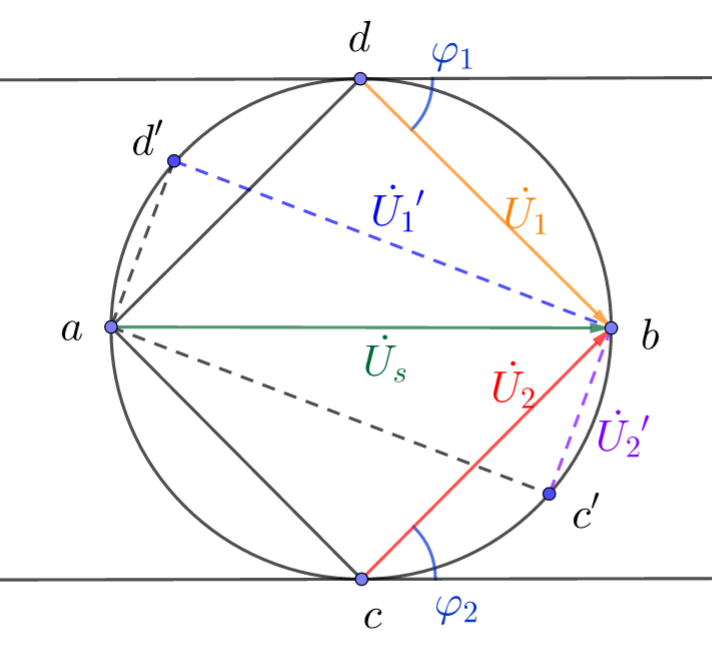
\includegraphics[width=3.5in]{TIM20180531102852.png}
\caption{\heiti\zihao{5}RC桥式分相电路裂二相相量图原理}\label{fig:1}
\end{figure}

图中,$U_1,U_2$为输出电压,$U_s$为输入电压,满足
\begin{equation}\label{1}
\left\{ 
\begin{array}{c}
\frac{U_1}{U_s}=\frac{1}{\sqrt{1+(\omega R_1C_1)^2}} \\
\frac{U_2}{U_s}=\frac{1}{\sqrt{1+\left(\frac{1}{\omega R_2C_2}\right)^2}}
\end{array} \right.  
\end{equation}
对输入电压$U_s$而言,输出电压$U_1,U_2$的相位为
\begin{equation}\label{2}
\left\{ 
\begin{array}{c}
\varphi_1=-arctan\omega R_1C_1 \\
\varphi_1=arctan\frac{1}{\omega R_2C_2}
\end{array} \right.  
\end{equation}
或
\begin{equation}\label{}
cot\varphi_2=\omega R_2C_2=-tan(\varphi_2+90\degree)
\end{equation}
由此
\begin{equation}\label{}
\varphi_2+90\degree=-arctan\omega R_2C_2
\end{equation}
若
\begin{equation}\label{}
R_1C_1=R_2C_2=RC
\end{equation}
则必有
\begin{equation}\label{}
\varphi_1-\varphi_2=90\degree
\end{equation}
一般而言,$\varphi_1$和$\varphi_2$与角频率$\omega$无关,但为使$U_1$和$U_2$数值相等,可令
\begin{equation}\label{tiaojian}
\omega R_1C_1=\omega R_2C_2=1
\end{equation}
而$U_s=220V,\omega =50Hz$,将(\ref{tiaojian})带入(\ref{1})(\ref{2}),理论上因有
\begin{equation}\label{jieguo1}
\left\{ 
\begin{array}{c}
U_1=\frac{1}{2}U_s \\
U_2=\frac{1}{2}U_s \\
\varphi_1=-45\degree\\
\varphi_1=45\degree
\end{array} \right.  
\end{equation}
取$R_1=R_2=1k\Omega ,C_1=C_2=3.183\mu F$得到如图\ref{fig:3}电路。
\begin{figure}[htbp]
\centering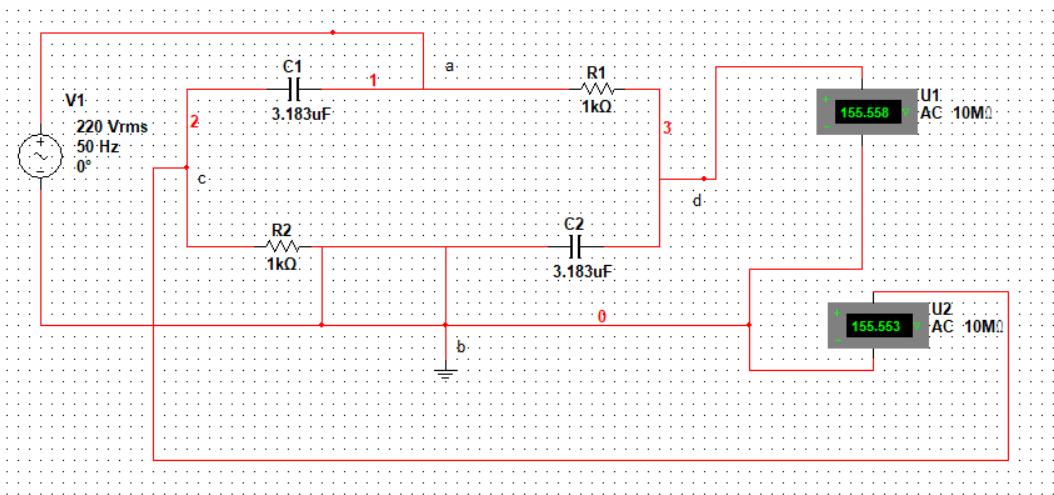
\includegraphics[width=\linewidth]{TIM20180531145325.png}
\caption{\heiti\zihao{5}multisim二项裂相电路仿真图}\label{fig:3}
\end{figure}
从中可以看出,空载输出电压分别为$U_1=155.558V,U_2=155.553V$,在误差允许范围内可以认为$U_1=U_2\in  \{ 150\times (1\pm 4\%)\}$;借助示波器测量输出电压波形情况如图\ref{fig:4},计算可得相位差为$2\times 180\degree\times 50Hz\times 5.076ms=91.368\degree\in \{90\degree\times (1\pm 2\%)\}$,二相电路裂相完成。
\begin{figure}[htbp]
\centering
\begin{tabular}{cc}
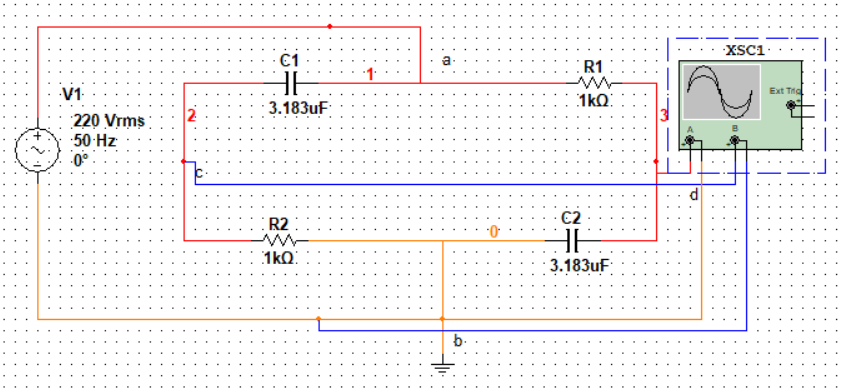
\includegraphics[width=0.48\linewidth]{TIM20180531151220.png}&
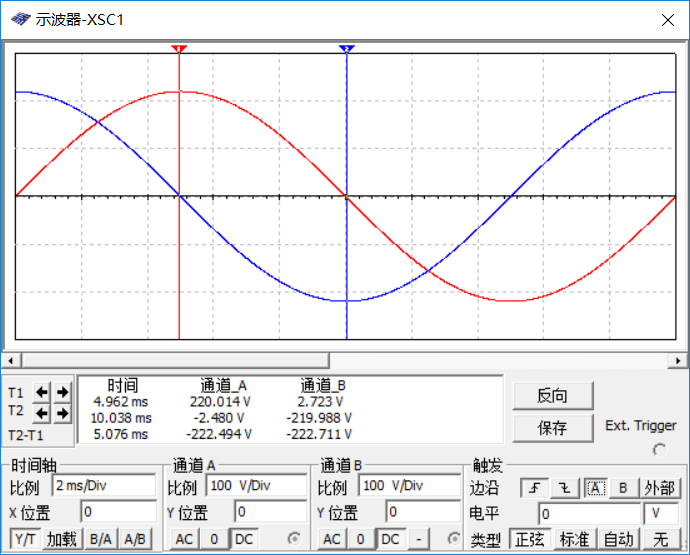
\includegraphics[width=0.48\linewidth]{TIM20180531151209.png}\\
(a)&(b)\\
\end{tabular}
\caption{\heiti\zihao{5}}\label{fig:4}
\end{figure}
\subsection{单向交流电源分裂为相位差为120\degree 的对称三相电源的裂相原理}
将单相电源$U_s$分裂成三相$U_1,U_2,U_3$互成$120\degree$的对称电压,其相量图原理如图\ref{fig:2}所示。
\begin{figure}[htbp]
\centering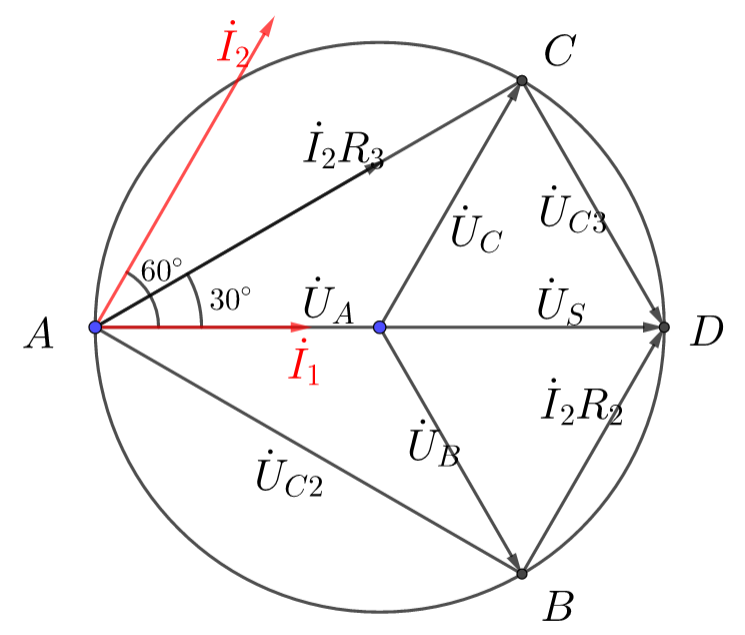
\includegraphics[width=3.5in]{TIM20180531133124.png}
\caption{\heiti\zihao{5}RC桥式分相电路裂三相相量图原理}\label{fig:2}
\end{figure}
电路的关键是元件参数。从相量图中可见,B和C的轨迹在圆周上变化。只要使得$I_2,I_1$相位差为$60\degree$;$I_3,I_1$相位差为$30\degree$,则可以使电压成对称三相电压。利用
\begin{equation}\label{}
\left\{ 
\begin{array}{c}
\frac{X_{C2}}{R_2}=tan60\degree \\
\frac{X_{C3}}{R_3}=tan30\degree
\end{array} \right.  
\end{equation}
取$R_1=R_2=R_3=1k\Omega,C_2=1.838\mu F,C_3=5.513\mu F$得到如图\ref{fig:3=}电路。
\begin{figure}[htbp]
\centering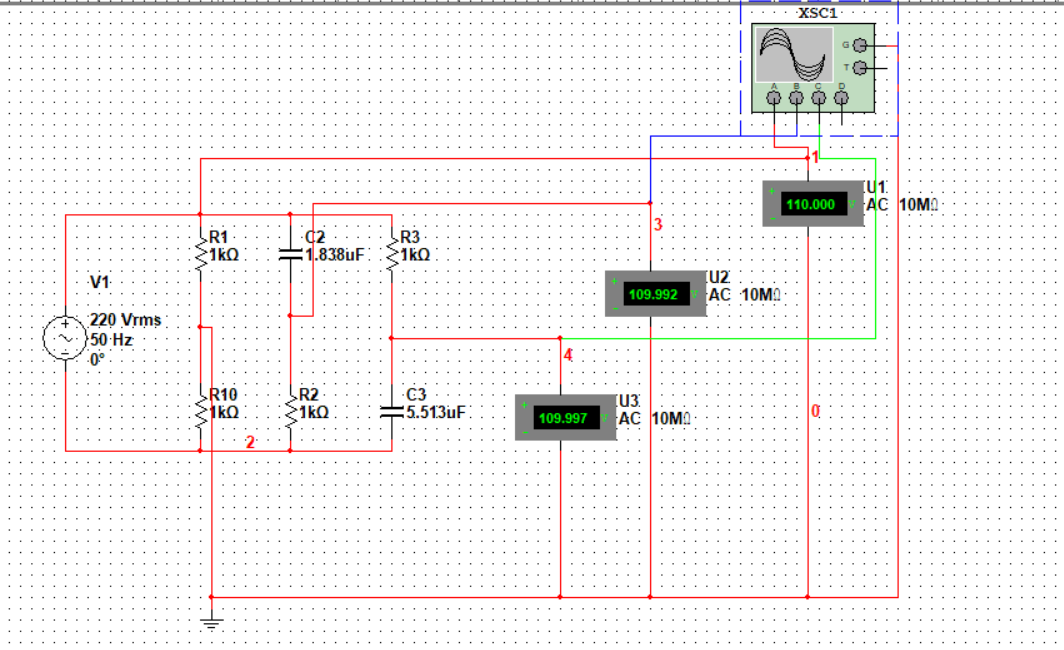
\includegraphics[width=\linewidth]{TIM20180531203831.png}
\caption{\heiti\zihao{5}multisim三项裂相电路仿真图}\label{fig:3=}
\end{figure}
从中可以看出,空载输出电压分别为$U_1=110.000V,U_2=109.992V,U_3=109.997V$,在误差允许范围内可以认为$U_1=U_2=U_3\in  \{ 110\times (1\pm 4\%)\}$;借助示波器测量输出电压波形情况如图\ref{fig:x},计算可得相位差分别为$2\times 180\degree\times 50Hz\times 6.667ms=120.006\degree\in \{120\degree\times (1\pm 2\%)\},360\degree -2\times 180\degree\times 50Hz\times 13.368ms=119.376\degree\in \{90\degree\times (1\pm 2\%)\},2\times 180\degree\times 50Hz\times 6.702ms=120.636\degree\in \{120\degree\times (1\pm 2\%)\}$,误差允许范围内认为相位差相同,三相电路裂相完成。
\begin{figure}[htbp]
\centering
\begin{tabular}{cc}
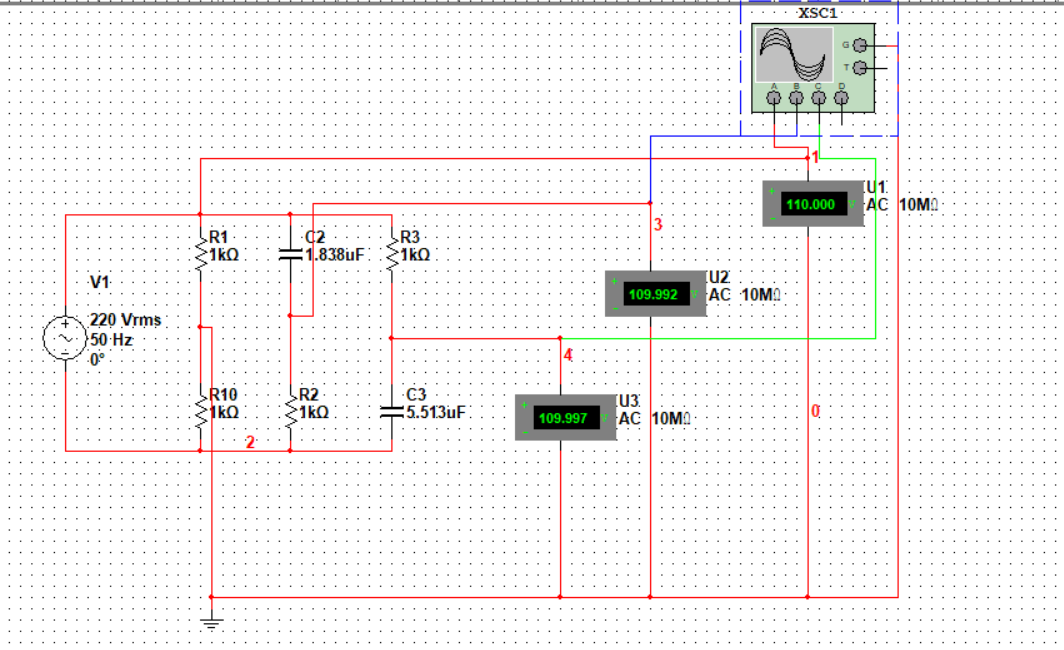
\includegraphics[width=0.48\linewidth]{TIM20180531203831.png}&
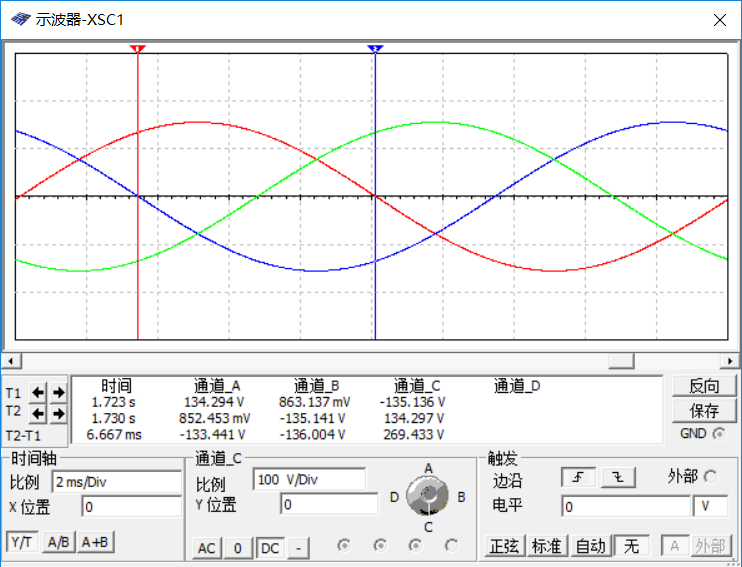
\includegraphics[width=0.48\linewidth]{TIM20180531203650.png}\\
(a)&(b)\\
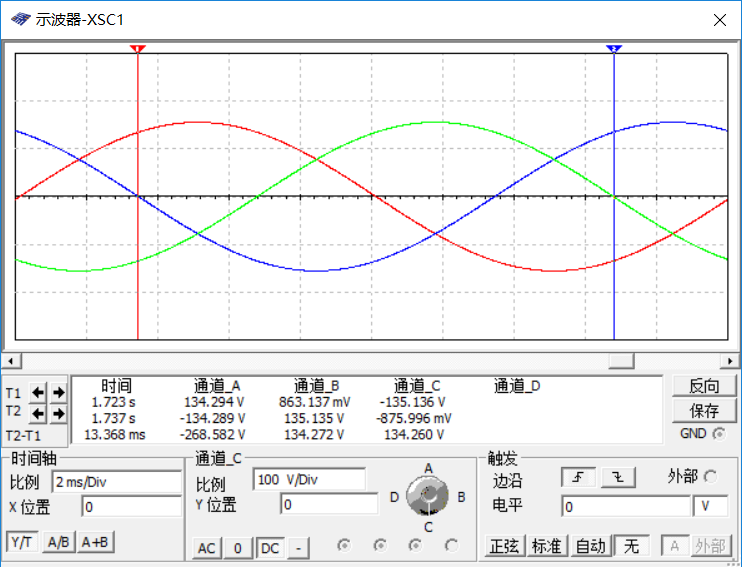
\includegraphics[width=0.48\linewidth]{TIM20180531203728.png}&
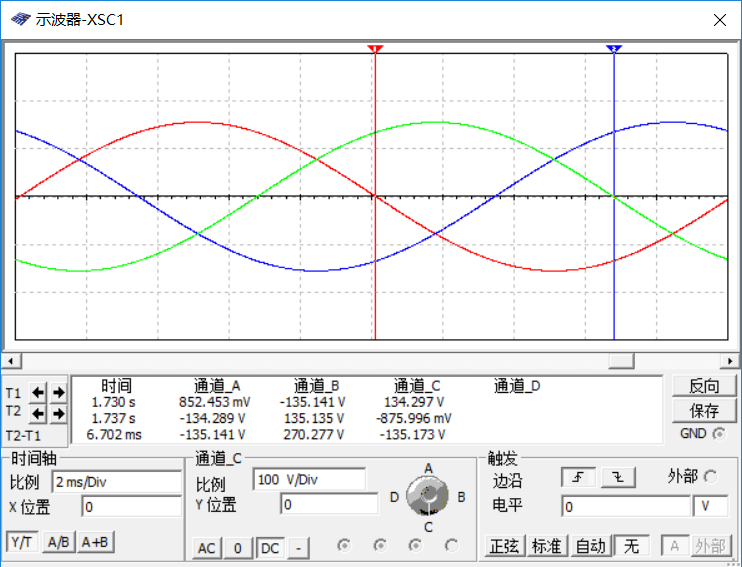
\includegraphics[width=0.48\linewidth]{TIM20180531203812.png}\\
(c)&(d)\\
\end{tabular}
\caption{\heiti\zihao{5}}\label{fig:x}
\end{figure}
\section{二相裂相电路相关数据的测量}
\subsection{电压-负载特性的数据测量与曲线绘制}
\subsubsection{电阻性负载的电压-负载特性}
按图\ref{fig:a1}连接线路,不断调节可变电阻参数,记录相应的数据见表\ref{tab:addlabel1}。从表中可以看出,无论负载的变化,二相相位差总大致相等。事实上,由于各相负载等值(对称),所以相位差不变,在之后的仿真中,不再单独测量、计算相位差。实验的仿真截图见图\ref{fig:x1},此时负载电阻取$1k\Omega$。
\begin{figure}[htbp]
\centering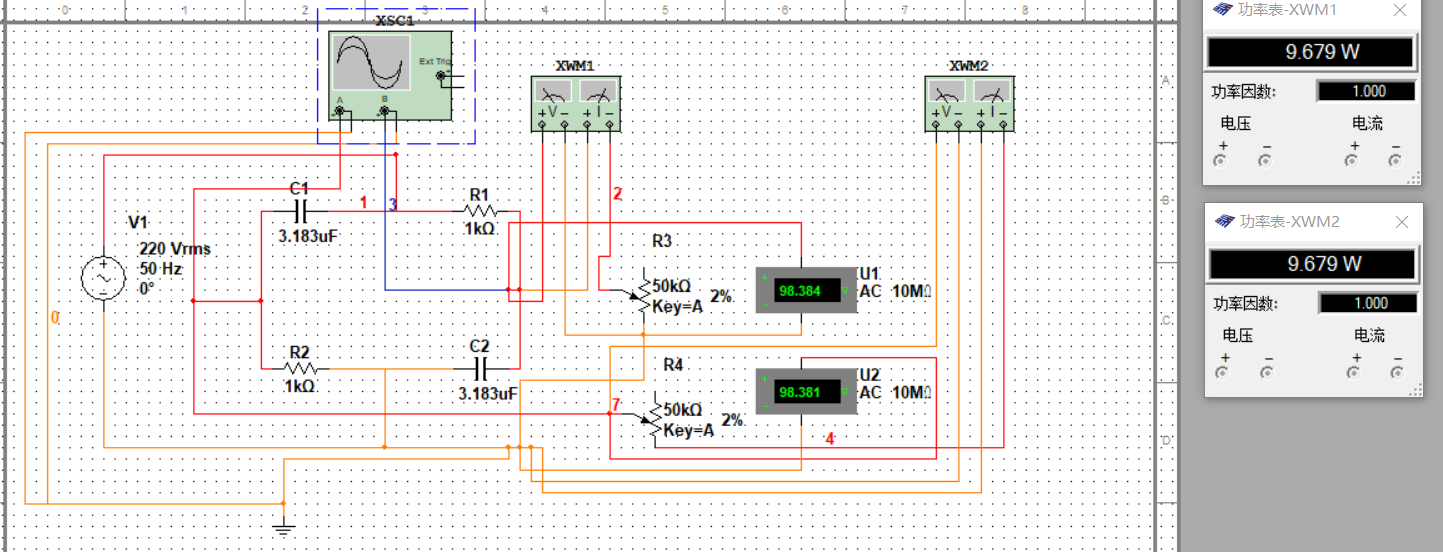
\includegraphics[width=\linewidth]{TIM20180531171555.png}
\caption{\heiti\zihao{5}}\label{fig:a1}
\end{figure}
\begin{table}[htbp]
  \centering
  \caption{\heiti\zihao{5}二相裂相电路电压、功率随电阻变化关系}
    \begin{tabular}{ccccccccc}
    \hline
    序号 & $R(\Omega)$ & $U_1(V)$ & $U_2(V)$ & $P_1(W)$ & $P_2(W)$ & $P_{all}(W)(=P_1+P_2)$ &$ T(ms)$  & $\Delta \varphi( \degree )$ \\
    \hline
1  & 100 & 19.918 & 19.917 & 3.967 & 3.967 & 7.934 & 5.057  & 91.026  \\
2  & 200 & 36.167 & 36.166 & 6.540 & 6.540 & 13.08 & 5.019  & 90.342  \\
3  & 300 & 49.468 & 49.467 & 8.157 & 8.157 & 16.314 & 4.943  & 88.974  \\
4  & 400 & 60.437 & 60.435 & 9.132 & 9.131 & 18.263 & 5.038  & 90.684  \\
5  & 500 & 69.568  & 69.566  & 9.679  & 9.679  & 19.358  & 4.962  & 89.316  \\
6  & 600 & 77.245 & 77.243 & 9.945 & 9.944 & 19.889 & 5.000  & 90.000  \\
7  & 800 & 89.348 & 89.345 & 9.979 & 9.978 & 19.957 & 4.981  & 89.658  \\
8  & 1000 & 98.384  & 98.381  & 9.679  & 9.679  & 19.358  & 5.000  & 90.000  \\
9  & 1500 & 113.156  & 113.152  & 8.541  & 8.540  & 17.081  & 5.038  & 90.684  \\
10 & 2000 & 122.030  & 122.026  & 7.446  & 7.445  & 14.891  & 5.038  & 90.684  \\
11 & 2500 & 127.830  & 127.864  & 6.540  & 6.540  & 13.080  & 5.076  & 91.368  \\
12 & 3000 & 131.995  & 131.947  & 5.808  & 5.807  & 11.615  & 5.057  & 91.026  \\
13 & 3500 & 135.062  & 135.058  & 5.212  & 5.212  & 10.424  & 5.095  & 91.710  \\
14 & 4000 & 137.428  & 137.424  & 4.722  & 4.721  & 9.443  & 5.019  & 90.342  \\
15 & 4500 & 139.280  & 139.303  & 4.313  & 4.312  & 8.625  & 4.905  & 88.290  \\
16 & 5000 & 140.799  & 140.831  & 3.967  & 3.967  & 7.934  & 5.076  & 91.368  \\
17 & 5500 & 142.102  & 142.098  & 3.671  & 3.670  & 7.341  & 4.924  & 88.632  \\
18 & 6000 & 143.169  & 143.165  & 3.416  & 3.416  & 6.832  & 5.019  & 90.342  \\
19 & 6500 & 144.043  & 144.038  & 3.194  & 3.193  & 6.387  & 5.038  & 90.684  \\
20 & 7000 & 144.866  & 144.861  & 2.998  & 2.998  & 5.996  & 5.057  & 91.026  \\
21 & 7500 & 145.511  & 145.547  & 2.825  & 2.825  & 5.650  & 4.962  & 89.316  \\
22 & 8000 & 146.155  & 146.150  & 2.670  & 2.670  & 5.340  & 5.000  & 90.000  \\
23 & 8500 & 146.690  & 146.685  & 2.532  & 2.531  & 5.063  & 4.943  & 88.974  \\
24 & 9000 & 147.167  & 147.162  & 2.406  & 2.406  & 4.812  & 4.924  & 88.632  \\
25 & 9500 & 147.596  & 147.591  & 2.293  & 2.293  & 4.586  & 5.019  & 90.342  \\
26 & 10000 & 147.983  & 147.978  & 2.190  & 2.190  & 4.380  & 5.057  & 91.026  \\
27 & 10500 & 148.288  & 148.329  & 2.096  & 2.095  & 4.191  & 5.038  & 90.684  \\
28 & 11000 & 148.654  & 148.612  & 2.009  & 2.009  & 4.018  & 4.981  & 89.658  \\
29 & 11500 & 148.947  & 148.943  & 1.929  & 1.929  & 3.858  & 5.019  & 90.342  \\
30 & 12000 & 149.216  & 149.212  & 1.855  & 1.855  & 3.710  & 5.057  & 91.026  \\
31 & 12500 & 149.464  & 149.460  & 1.787  & 1.787  & 3.574  & 5.000  & 90.000  \\
32 & 13000 & 149.694  & 149.689  & 1.724  & 1.724  & 3.448  & 4.962  & 89.316  \\
33 & 13500 & 149.907  & 149.902  & 1.665  & 1.664  & 3.329  & 4.981  & 89.658  \\
34 & 14000 & 150.066  & 150.100  & 1.609  & $1.609$  & 3.218  & 5.076  & 91.368  \\
    35 &$\infty$ & 155.558  & 155.553  & 24.197n & 0  &  24.197n  & 5.076  & 91.368  \\
    \hline
    \end{tabular}%
  \label{tab:addlabel1}%
\end{table}%
\begin{figure}[htbp]
\centering
\begin{tabular}{cc}
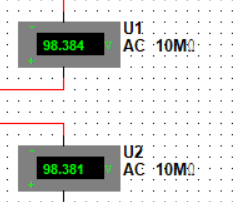
\includegraphics[width=0.45\linewidth]{TIM20180531171612.png}&
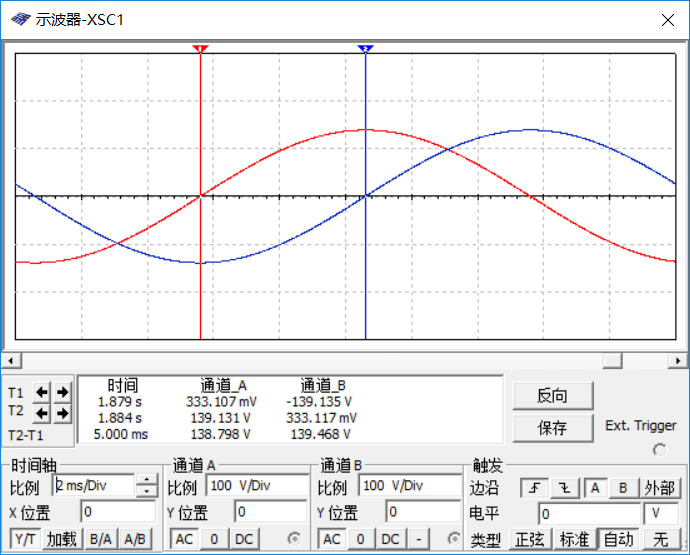
\includegraphics[width=0.45\linewidth]{TIM20180531171724.png}\\
(a)&(b)\\
\end{tabular}
\caption{\heiti\zihao{5}}\label{fig:x1}
\end{figure}

由得到的数据,借助EXCEL可以绘制电压-负载特性曲线,其结果如图\ref{fig:a11}。\par
从中可以看出,$U_1,U_2$的曲线几乎完全重合,且随着负载电阻值增加,电压值不断增大,最终趋近于空载电压。
\begin{figure}[htbp]
\centering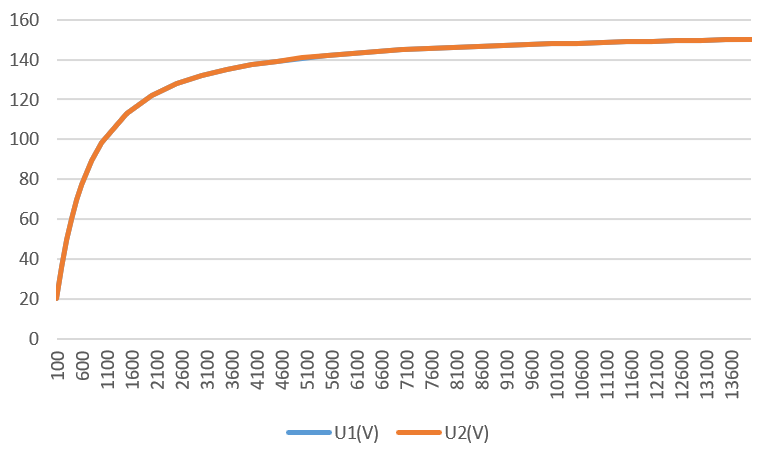
\includegraphics[width=0.8\linewidth]{TIM20180531191154.png}
\caption{\heiti\zihao{5}电阻性负载电压-负载特性曲线}\label{fig:a11}
\end{figure}
\subsubsection{容性负载的电压-负载特性}
当负载为容性时,按图\ref{fig:a12}连接线路,同样不断调节可变电容参数,记录相应的数据见表\ref{tab:addlabel2},实验的仿真截图见图\ref{fig:x11},此时负载容抗取$0.8\mu F$。
\begin{figure}[htbp]
\centering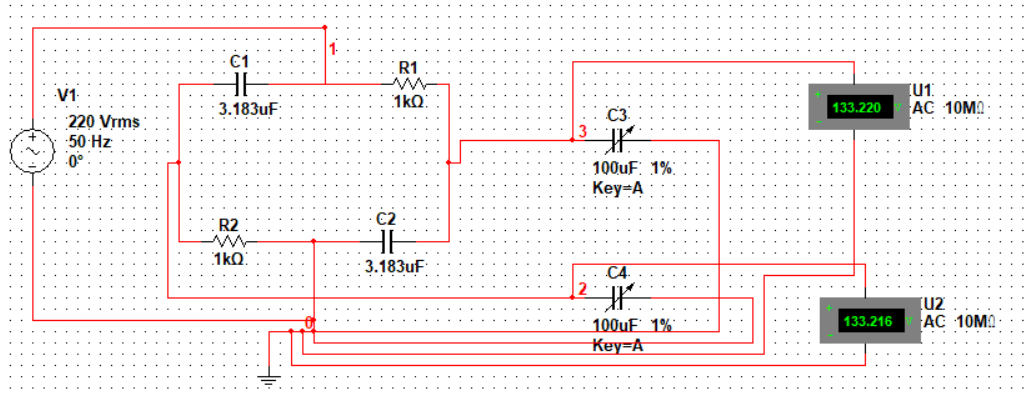
\includegraphics[width=\linewidth]{TIM20180531183801.png}
\caption{\heiti\zihao{5}}\label{fig:a12}
\end{figure}
\begin{figure}[htbp]
\centering
\begin{tabular}{cc}
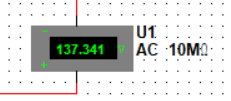
\includegraphics[width=0.4\linewidth]{TIM20180607115514.png}&
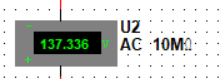
\includegraphics[width=0.4\linewidth]{TIM20180607115606.png}\\
(a)&(b)\\
\end{tabular}
\caption{\heiti\zihao{5}}\label{fig:x11}
\end{figure}

由表中的数据,借助EXCEL绘制电压-负载特性曲线,其结果如图\ref{fig:a121}。\par
\begin{figure}[htbp]
\centering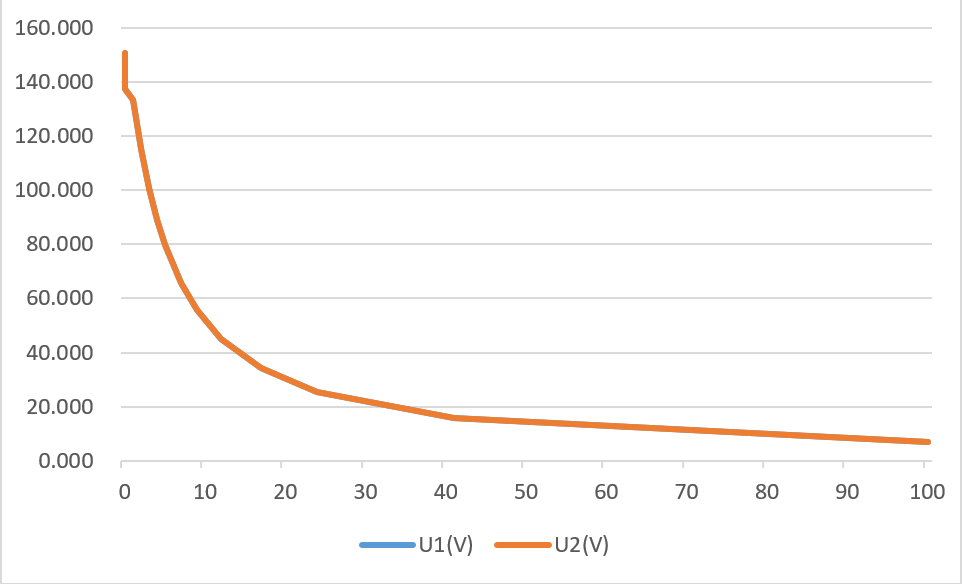
\includegraphics[width=0.8\linewidth]{TIM20180531191032.png}
\caption{\heiti\zihao{5}容性负载电压-负载特性曲线}\label{fig:a121}
\end{figure}
从中可以看出,$U_1,U_2$的曲线同样几乎完全重合,而随着负载容值增加,电压值不断减小。

\twocolumn
\begin{table}[htbp]
  \centering
  \caption{\heiti\zihao{5}二相裂相电路电压随电容变化关系}
    \begin{tabular}{cccc}
    \hline
   序号& $C(\mu F)$  & $U_1(V) $& $U_2(V)$ \\
        \hline
    1  & 0.2 & 150.750  & 150.746  \\
    2  & 0.4 & 146.108  & 146.103  \\
    3  & 0.6 & 141.637  & 141.632  \\
    4  & 0.8 & 137.341  & 137.336  \\
    5  & 1  & 133.220  & 133.216  \\
    6  & 2  & 115.129  & 115.126  \\
    7  & 3  & 100.696  & 100.396  \\
    8  & 4  & 89.130  & 89.128  \\
    9  & 5  & 79.755  & 79.753  \\
    10 & 7  & 65.637  & 65.635  \\
    11 & 9  & 55.613  & 55.594  \\
    12 & 12 & 45.129  & 45.140  \\
    13 & 17 & 34.264  & 34.272  \\
    14 & 24 & 25.587  & 25.586  \\
    15 & 41 & 15.809  & 15.808  \\
    16 & 100 & 6.784  & 6.783  \\
     \hline
    \end{tabular}%
  \label{tab:addlabel2}%
\end{table}%
% Table generated by Excel2LaTeX from sheet '裂二相电路'
\begin{table}[htbp]
  \centering
  \caption{\heiti\zihao{5}二相裂相电路电压随电感变化关系}
    \begin{tabular}{cccc}
        \hline
   序号 & $L(mH)$  & $U_1(V)$ & $U_2(V)$ \\
        \hline
    1  & 50 & 3.510  & 3.510  \\
    2  & 100 & 7.132  & 7.132  \\
    3  & 200 & 14.717  & 14.716  \\
    4  & 250 & 18.684  & 18.677  \\
    5  & 350 & 26.974  & 26.973  \\
    6  & 450 & 35.741  & 35.740  \\
    7  & 500 & 40.303  & 40.302  \\
    8  & 550 & 44.982  & 44.969  \\
    9  & 650 & 54.680  & 54.679  \\
    10 & 750 & 64.784  & 64.783  \\
    11 & 850 & 75.307  & 75.305  \\
    12 & 950 & 86.120  & 86.118  \\
    13 & 1000 & 91.594  & 91.591  \\
    14 & 1500 & 146.326  & 146.360  \\
    15 & 2000 & 189.334  & 189.329  \\
    16 & 2500 & 212.199  & 212.193  \\
    17 & 2700 & 216.481  & 216.474  \\
    18 & 2800 & 217.947  & 217.940  \\
    19 & 2900 & 218.937  & 218.930  \\
    20 & 3000 & 219.569  & 219.506  \\
    21 & 3100 & 219.899  & 219.892  \\
    22 & 3200 & 219.975  & 219.968  \\
    23 & 3300 & 219.840  & 219.834  \\
    24 & 3400 & 219.532  & 219.469  \\
    25 & 3500 & 219.083  & 219.076  \\
    26 & 4500 & 211.127  & 211.120  \\
    27 & 5000 & 206.755  & 206.749  \\
    28 & 6000 & 199.131  & 199.125  \\
    29 & 7500 & 190.659  & 190.653  \\
    30 & 10000 & 181.771  & 181.765  \\
    31 & 15000 & 172.807  & 172.802  \\
    32 & 20000 & 168.378  & 168.331  \\
    33 & 40000 & 161.864  & 161.860  \\
    34 & 100000 & 158.053  & 158.048  \\
            \hline
    \end{tabular}%
  \label{tab:addlabel3}%
\end{table}%
\onecolumn
\subsubsection{感性负载的电压-负载特性}
当负载为感性时,按图\ref{fig:a12a}连接线路,同样不断调节可变电感参数,记录相应的数据见表\ref{tab:addlabela},实验的仿真截图见图\ref{fig:x11a},此时负载感抗取$950mH$。
\begin{figure}[htbp]
\centering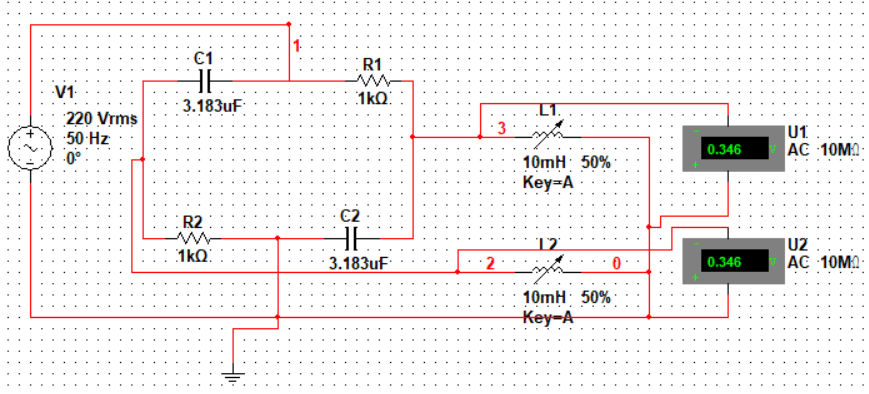
\includegraphics[width=\linewidth]{TIM20180601152857.png}
\caption{\heiti\zihao{5}}\label{fig:a12a}
\end{figure}
\begin{figure}[htbp]
\centering
\begin{tabular}{cc}
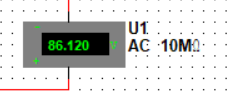
\includegraphics[width=0.4\linewidth]{TIM20180607120314.png}&
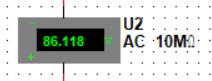
\includegraphics[width=0.4\linewidth]{TIM20180607120357.png}\\
(a)&(b)\\
\end{tabular}
\caption{\heiti\zihao{5}}\label{fig:x11a}
\end{figure}

由表中的数据,借助EXCEL绘制电压-负载特性曲线,其结果如图\ref{fig:a121x}。\par
\begin{figure}[htbp]
\centering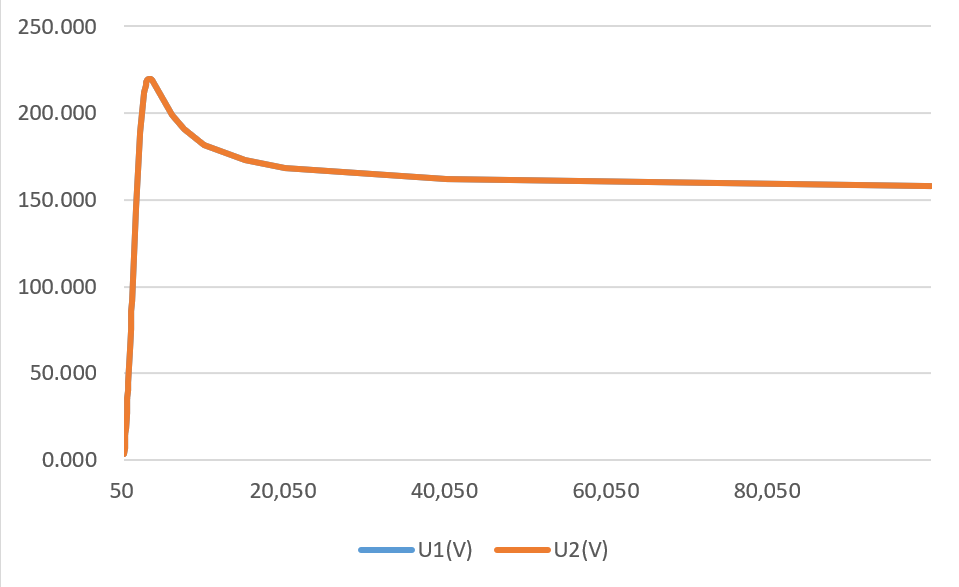
\includegraphics[width=0.8\linewidth]{TIM20180531195752.png}
\caption{\heiti\zihao{5}感性负载电压-负载特性曲线}\label{fig:a121x}
\end{figure}
从图中可以看出,$U_1,U_2$基本相等,而随着负载电感值的增加,电压值先快速增加,在$L=3200mH$时达到最大,之后逐渐减小到空载电压。
\subsection{功率-负载特性的数据测量与曲线绘制}
事实上,在测量电阻的电压负载特性时,也同步测量了其功率。按如图\ref{fig:a1}所示电路连接,测得的数据见表\ref{tab:addlabel1},实验的仿真截图见图\ref{fig:x11a8},此时负载电阻取$1k\Omega$。
\begin{figure}[htbp]
\centering
\begin{tabular}{cc}
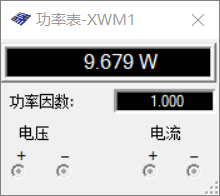
\includegraphics[width=0.3\linewidth]{TIM20180607120801.png}&
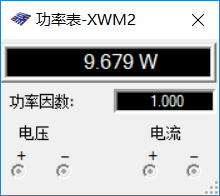
\includegraphics[width=0.3\linewidth]{TIM20180607120828.png}\\
(a)&(b)\\
\end{tabular}
\caption{\heiti\zihao{5}}\label{fig:x11a8}
\end{figure}

通过表中的数据,借助EXCEL绘制功率-负载特性曲线,其结果如图\ref{fig:a121xs}。
\begin{figure}[htbp]
\centering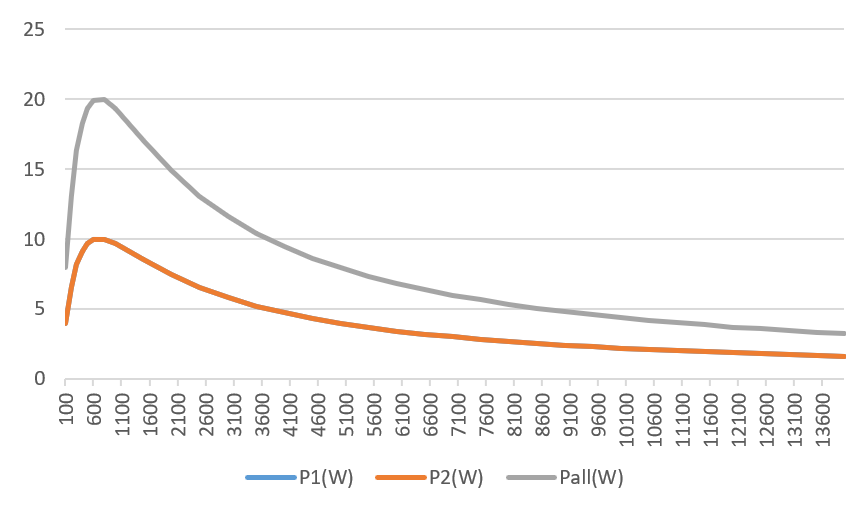
\includegraphics[width=0.8\linewidth]{TIM20180531191301.png}
\caption{\heiti\zihao{5}功率-负载特性曲线}\label{fig:a121xs}
\end{figure}
从图中可以看出,$P_1,P_2$大致相等。随着负载电阻值的增加,$P_1,P_2,P_{all}$功率均先快速增加,在$R=800\Omega$左右时达到最大,之后逐渐减小。

借助功率-负载曲线图可以推断,当R无限大时,功率将变为0。即证明电路在空载时功耗最小。
\section{三相裂相电路相关数据的测量}
\subsection{电压-负载特性的数据测量与曲线绘制}
\subsubsection{电阻性负载的电压-负载特性}
按图\ref{fig:a19}连接线路,不断调节可变电阻参数,记录相应的数据见表\ref{tab:addlabela}。实验的仿真截图见图\ref{fig:a19xx},此时负载电阻取$500\Omega$。
\begin{figure}[htbp]
\centering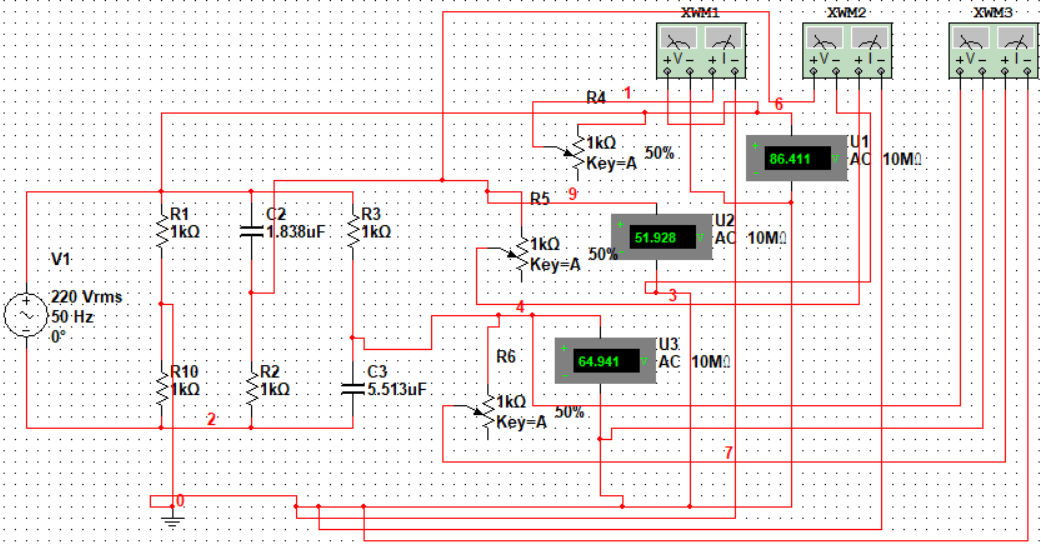
\includegraphics[width=\linewidth]{TIM20180607123951.png}
\caption{\heiti\zihao{5}}\label{fig:a19}
\end{figure}
\begin{figure}[htbp]
\begin{tabular}{ccc}
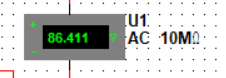
\includegraphics[width=0.3\linewidth]{TIM20180607123059.png}&
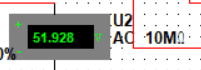
\includegraphics[width=0.3\linewidth]{TIM20180607123140.png}&
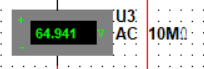
\includegraphics[width=0.3\linewidth]{TIM20180607123158.png}\\
(a)&(b)&(c)\\
\end{tabular}
\caption{\heiti\zihao{5}}\label{fig:a19xx}
\end{figure}

\begin{table}[htbp]
  \centering
  \caption{\heiti\zihao{5}三相裂相电路电压、功率随电阻变化关系}
    \begin{tabular}{ccccccccc}
    \hline
    序号 & $R(\Omega)$  & $U_1(V)$ & $U_2(V)$ & $U_3(V)$ & $P_1(W) $&$ P_2(W) $& $P_3(W) $& $P_{all}(W)=P_1+P_ 2+P_3$\\
        \hline
    1  & 50 & 24.034  & 9.937  & 15.805  & 11.553  & 1.975  & 4.996  & 18.524  \\
    2  & 100 & 40.534  & 18.024  & 26.949  & 16.430  & 3.249  & 7.269  & 26.948  \\
    3  & 150 & 50.322  & 24.709  & 35.297  & 18.251  & 4.070  & 8.306  & 30.627  \\
    4  & 200 & 61.083  & 30.343  & 41.882  & 18.565  & 4.604  & 8.770  & 31.939  \\
    5  & 210 & 62.568  & 31.367  & 43.043  & 18.642  & 4.685  & 8.822  & 32.149  \\
    6  & 220 & 63.978  & 32.361  & 44.161  & 18.606  & 4.760  & 8.865  & 32.231  \\
    7  & 230 & 65.320  & 33.325  & 45.239  & 18.551  & 4.829  & 8.898  & 32.278  \\
    8  & 240 & 66.598  & 34.263  & 46.278  & 18.480  & 4.891  & 8.924  & 32.295  \\
    9  & 250 & 67.815  & 35.174  & 47.252  & 18.396  & 4.949  & 8.942  & 32.287  \\
    10 & 300 & 73.133  & 39.373  & 51.839  & 17.828  & 5.168  & 8.957  & 31.953  \\
    11 & 400 & 80.961  & 46.346  & 59.195  & 16.387  & 5.370  & 8.760  & 30.517  \\
    12 & 500 & 86.411  & 51.928  & 64.941  & 14.934  & 5.939  & 8.435  & 29.308  \\
    13 & 650 & 92.002  & 58.520  & 71.586  & 13.022  & 5.269  & 7.884  & 26.175  \\
    14 & 1000 & 99.152  & 68.958  & 81.734  & 9.831  & 4.755  & 6.680  & 21.266  \\
    15 & 1500 & 103.715  & 77.852  & 89.820  & 7.171  & 4.041  & 5.378  & 16.590  \\
    16 & 2000 & 105.894  & 83.423  & 94.489  & 5.607  & 3.480  & 4.464  & 13.551  \\
    17 & 2500 & 107.106  & 87.281  & 97.489  & 4.589  & 3.040  & 3.802  & 11.431  \\
    18 & 4500 & 108.927  & 95.500  & 103.111  & 2.637  & 2.027  & 2.363  & 7.027  \\
    19 & 5000 & 109.110  & 96.689  & 103.828  & 2.381  & 1.870  & 2.156  & 6.407  \\
    20 & 7000 & 109.516  & 99.962  & 105.664  & 1.713  & 1.427  & 1.595  & 4.735  \\
    21 & 7500 & 109.574  & 100.542  & 105.968  & 1.601  & 1.348  & 1.497  & 4.446  \\
    22 & 10000 & 109.751  & 102.656  & 107.022  & 1.205  & 1.054  & 1.145  & 3.404  \\
    23 & 12500 & 109.837  & 103.994  & 107.644  & 0.965  & 0.865  & 0.926  & 2.756  \\
    24 & 25000 & 109.957  & 106.852  & 108.854  & 0.483  & 0.456  & 0.473  & 1.412  \\
    25 & 50000 & 109.989  & 108.384  & 109.436  & 0.241  & 0.234  & 0.239  & 0.714  \\
    26 & $\infty$ & 110 & 109.992 & 109.997 & 0  & 0  & 0  & 0 \\
        \hline
    \end{tabular}%
  \label{tab:addlabela}%
\end{table}%
由得到的数据,借助EXCEL可以绘制电压-负载特性曲线,其结果如图\ref{fig:b11}。\par
从图中可以看出,$U_1,U_2,U_3$的曲线开始时几乎完全重合,到某一电阻值逐渐分离,在$R=5050\Omega$左右时达到最大差距位置,之后三者皆靠近空载电压,且随着负载电阻值增加,电压值不断增大。
\begin{figure}[htbp]
\centering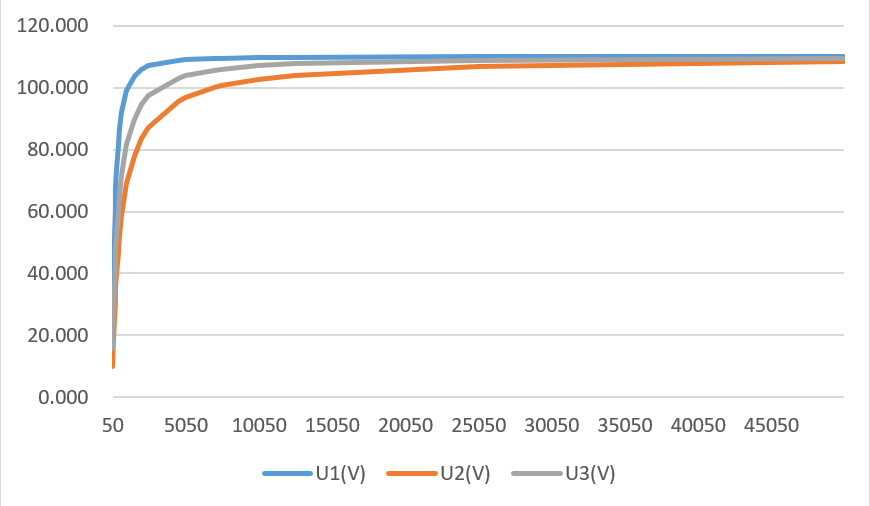
\includegraphics[width=0.8\linewidth]{TIM20180531233136.png}
\caption{\heiti\zihao{5}电阻性负载电压-负载特性曲线}\label{fig:b11}
\end{figure}
\subsubsection{容性负载的电压-负载特性}
当负载为容性时,按图\ref{fig:a120}连接线路,同样不断调节可变电容参数,记录相应的数据见表\ref{tab:addlabel23},实验的仿真截图见图\ref{fig:x11m},此时负载容抗取$10\mu F$。
\begin{figure}[htbp]
\centering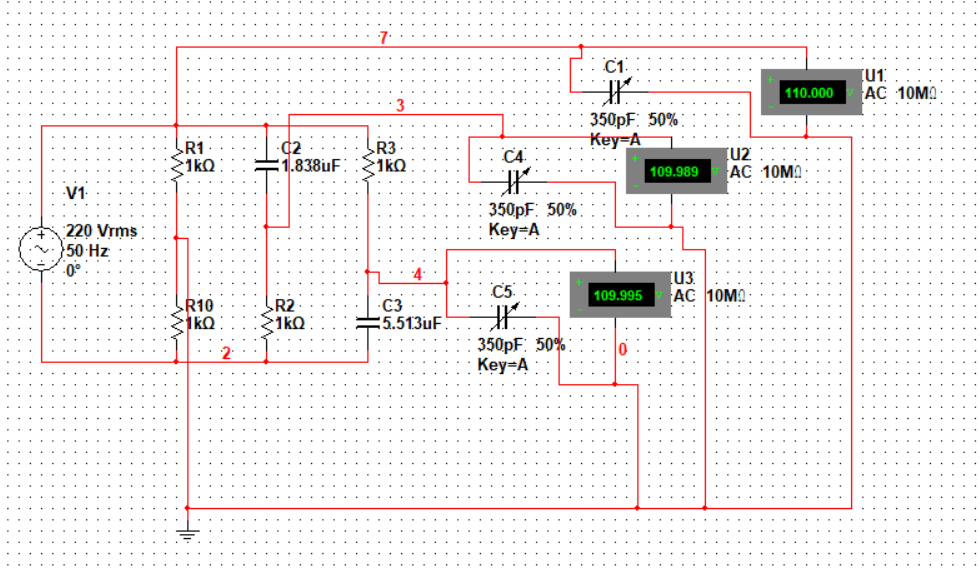
\includegraphics[width=\linewidth]{TIM20180531233912.png}
\caption{\heiti\zihao{5}}\label{fig:a120}
\end{figure}
\begin{figure}[htbp]
\centering
\begin{tabular}{ccc}
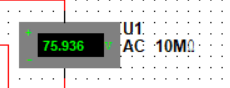
\includegraphics[width=0.3\linewidth]{TIM20180607131314.png}&
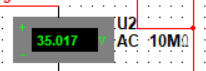
\includegraphics[width=0.3\linewidth]{TIM20180607131327.png}&
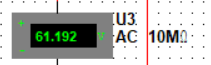
\includegraphics[width=0.3\linewidth]{TIM20180607131344.png}\\
(a)&(b)&(c)\\
\end{tabular}
\caption{\heiti\zihao{5}}\label{fig:x11m}
\end{figure}

由表中的数据,借助EXCEL绘制电压-负载特性曲线,其结果如图\ref{fig:a121o}。\par
\begin{figure}[htbp]
\centering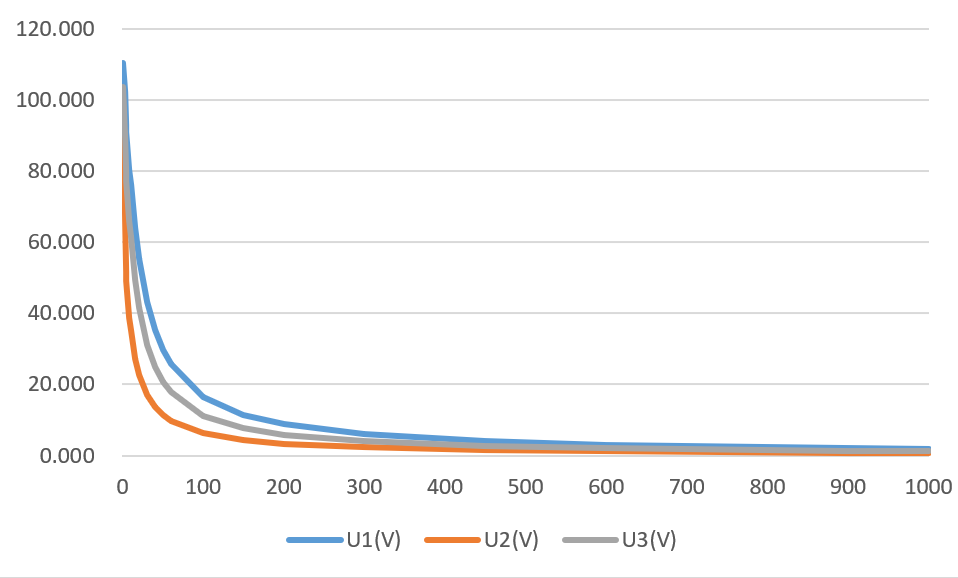
\includegraphics[width=0.8\linewidth]{TIM20180601004549.png}
\caption{\heiti\zihao{5}容性负载电压-负载特性曲线}\label{fig:a121o}
\end{figure}
从中可以看出,$U_1,U_2,U_3$的曲线同样开始时几乎重合,从某一电容值开始逐渐分离,在$C=50\mu F$左右时达到最大差距位置,之后三者皆靠近空载电压,且随着负载电容值增加,电压值不断减小。

\twocolumn
\begin{table}[htbp]
  \centering
  \caption{\heiti\zihao{5}三相裂相电路电压随电容变化关系}
    \begin{tabular}{ccccc}
    \hline
    序号 & $C(\mu F)$ & $U_1(V)$ & $U_2(V)$ & $U_3(V)$ \\
        \hline
    1  & 0.5 & 110.257  & 101.319  & 103.745  \\
    2  & 3  & 102.079  & 65.362  & 89.009  \\
    3  & 5  & 93.034  & 51.504  & 79.380  \\
    4  & 5.5 & 90.986  & 49.030  & 77.170  \\
    5  & 8.5 & 80.372  & 38.535  & 65.800  \\
    6  & 10 & 75.936  & 35.017  & 61.192  \\
    7  & 15 & 64.034  & 27.246  & 49.481  \\
    8  & 20 & 55.213  & 22.549  & 41.444  \\
    9  & 30 & 43.073  & 16.943  & 31.181  \\
    10 & 40 & 35.186  & 13.623  & 24.935  \\
    11 & 50 & 29.690  & 11.403  & 20.748  \\
    12 & 60 & 25.655  & 9.808  & 17.754  \\
    13 & 100 & 16.572  & 6.291  & 11.231  \\
    14 & 150 & 11.468  & 4.343  & 7.686  \\
    15 & 200 & 8.763  & 3.316  & 5.840  \\
    16 & 300 & 5.951  & 2.251  & 3.943  \\
    17 & 450 & 4.017  & 1.519  & 2.651  \\
    18 & 600 & 3.031  & 1.146  & 1.997  \\
    19 & 900 & 2.033  & 0.769  & 1.337  \\
    20 & 1000 & 1.832  & 0.693  & 1.204  \\
        \hline
    \end{tabular}%
  \label{tab:addlabel23}%
\end{table}%
\begin{table}[htbp]
  \centering
  \caption{\heiti\zihao{5}三相裂相电路电压随电感变化关系}
    \begin{tabular}{ccccc}
    \hline
    序号 & $L(mh)$ & $U_1(V)$ & $U_2(V)$ & $U_3(V)$ \\
  \hline
    1  & 50 & 9.646  & 3.650  & 6.198  \\
    2  & 100 & 20.302  & 7.710  & 12.790  \\
    3  & 150 & 31.913  & 12.195  & 19.692  \\
    4  & 200 & 44.323  & 17.090  & 26.761  \\
    5  & 250 & 57.252  & 22.334  & 33.790  \\
    6  & 300 & 70.299  & 27.822  & 40.520  \\
    7  & 350 & 82.979  & 33.405  & 46.676  \\
    8  & 400 & 94.803  & 38.920  & 52.011  \\
    9  & 450 & 105.367  & 44.215  & 56.358  \\
    10 & 500 & 114.418  & 49.177  & 59.662  \\
    11 & 550 & 121.884  & 53.751  & 61.977  \\
    12 & 650 & 132.461  & 61.748  & 64.232  \\
    13 & 800 & 140.539  & 71.577  & 64.461  \\
    14 & 1000 & 144.429  & 82.622  & 64.867  \\
    15 & 1500 & 147.340  & 105.316  & 81.270  \\
    16 & 2000 & 147.959  & 118.935  & 104.217  \\
    17 & 2500 & 145.804  & 124.053  & 119.760  \\
    18 & 3000 & 142.135  & 124.743  & 128.047  \\
    19 & 3500 & 138.179  & 121.674  & 134.071  \\
    20 & 4000 & 134.492  & 122.716  & 133.640  \\
    21 & 4500 & 131.238  & 121.674  & 134.071  \\
    22 & 5000 & 128.430  & 120.847  & 133.856  \\
    23 & 5500 & 126.029  & 120.220  & 133.297  \\
    24 & 6000 & 123.983  & 119.749  & 132.556  \\
    25 & 7000 & 120.753  & 119.111  & 130.867  \\
    26 & 10000 & 115.358  & 118.075  & 126.150  \\
  \hline
    \end{tabular}%
  \label{tab:addlabelaq}%
\end{table}%
\onecolumn
\subsubsection{感性负载的电压-负载特性}
当负载为感性时,按图\ref{fig:a12aq}连接线路,同样不断调节可变电感参数,记录相应的数据见表\ref{tab:addlabelaq},实验的仿真截图见图\ref{fig:x11aq},此时负载感抗取$5000mH$。
\begin{figure}[htbp]
\centering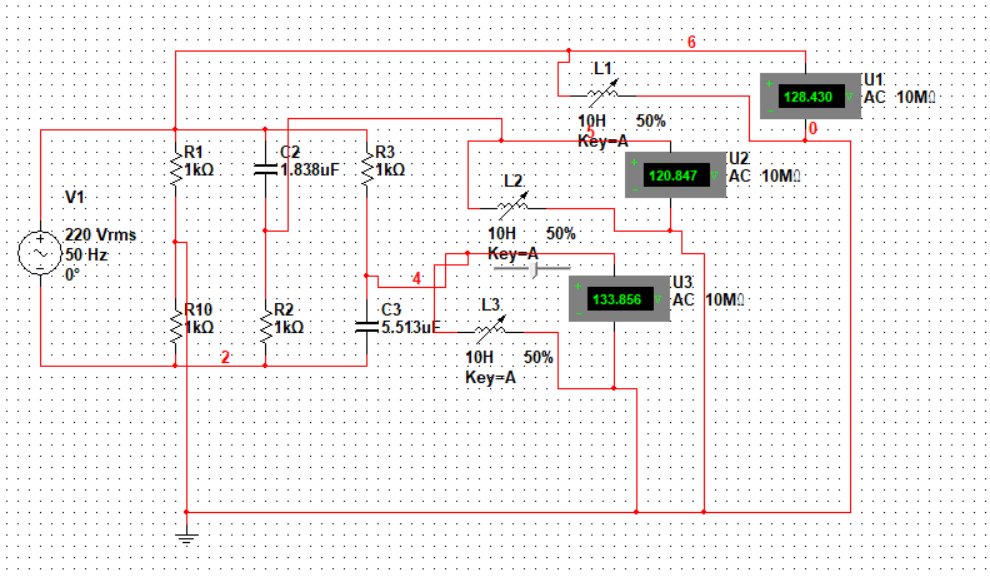
\includegraphics[width=\linewidth]{TIM20180601014335.png}
\caption{\heiti\zihao{5}}\label{fig:a12aq}
\end{figure}
\begin{figure}[htbp]
\centering
\begin{tabular}{ccc}
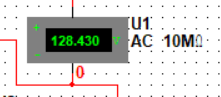
\includegraphics[width=0.3\linewidth]{TIM20180607122358.png}&
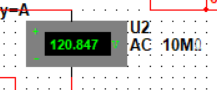
\includegraphics[width=0.3\linewidth]{TIM20180607122421.png}&
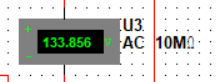
\includegraphics[width=0.3\linewidth]{TIM20180607122638.png}\\
(a)&(b)&(c)\\
\end{tabular}
\caption{\heiti\zihao{5}}\label{fig:x11aq}
\end{figure}

由表中的数据,借助EXCEL绘制电压-负载特性曲线,其结果如图\ref{fig:a121xq}。\par
\begin{figure}[htbp]
\centering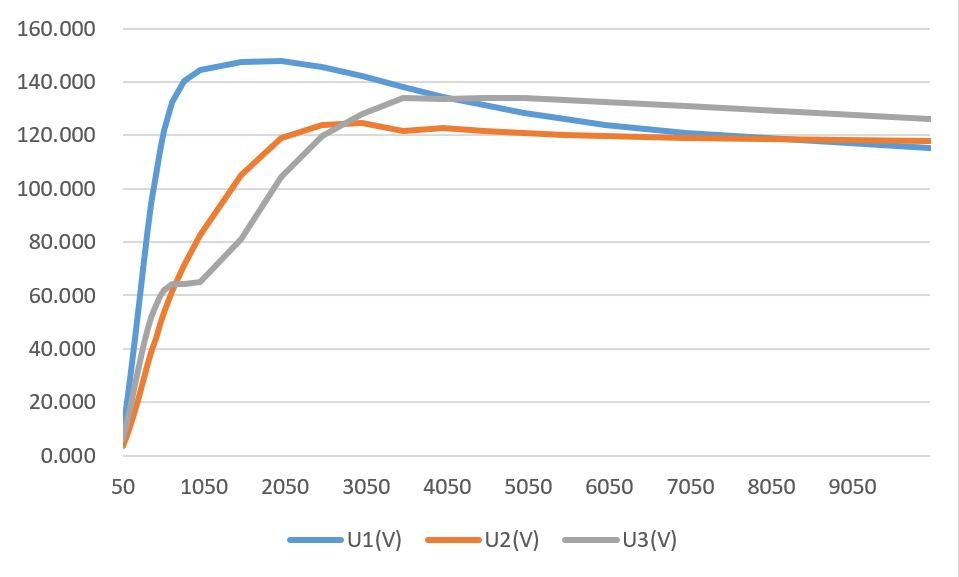
\includegraphics[width=0.8\linewidth]{TIM20180601015006.png}
\caption{\heiti\zihao{5}感性负载电压-负载特性曲线}\label{fig:a121xq}
\end{figure}
从图中可以看出,$U_1,U_2,U_3$总体趋势大致相同,均为先增大后减小并趋于空载电压。但在低电感区,三者的电压差距较大;高电感区,电压差距逐渐减小。
\subsection{功率-负载特性的数据测量与曲线绘制}
在测量电阻的电压负载特性时,同样同步测量其功率。按如图\ref{fig:a19}所示电路连接,测得的数据见表\ref{tab:addlabela},实验的仿真截图见图\ref{fig:x11a8xx},此时负载电阻取$500\Omega$。
\begin{figure}[htbp]
\centering
\begin{tabular}{ccc}
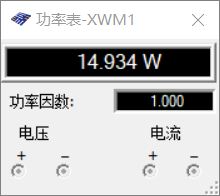
\includegraphics[width=0.3\linewidth]{TIM20180607130156.png}&
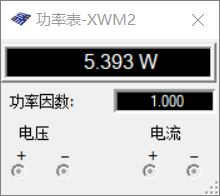
\includegraphics[width=0.3\linewidth]{TIM20180607130226.png}&
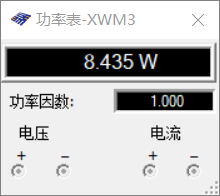
\includegraphics[width=0.3\linewidth]{TIM20180607130252.png}\\
(a)&(b)&(c)\\
\end{tabular}
\caption{\heiti\zihao{5}}\label{fig:x11a8xx}
\end{figure}

通过表中的数据,借助EXCEL绘制功率-负载特性曲线,其结果如图\ref{fig:a121xss}。
\begin{figure}[htbp]
\centering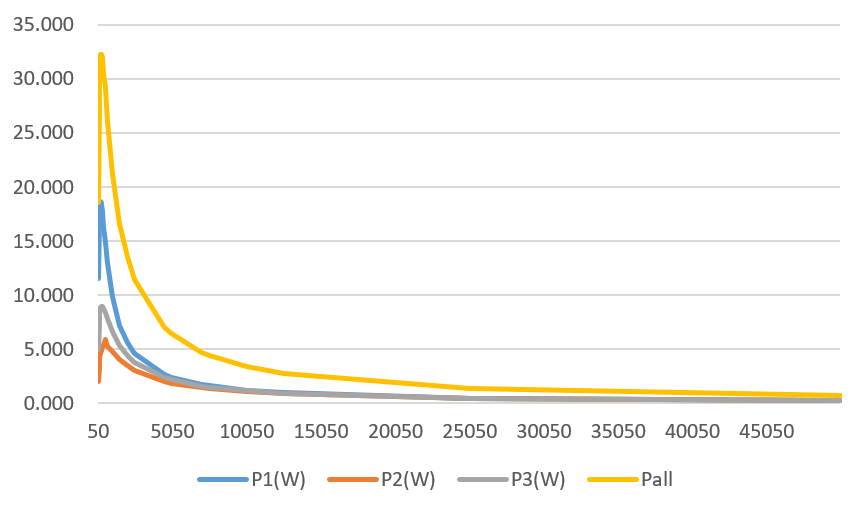
\includegraphics[width=0.8\linewidth]{TIM20180531233316.png}
\caption{\heiti\zihao{5}功率-负载特性曲线}\label{fig:a121xss}
\end{figure}
从图中可以看出,$P_1,P_2$开始时数值有一定差异,但变化趋势大致相同;$10k\Omega$后,$P_1,P_2,P_3$曲线几乎重合。随着负载电阻值的增加,$P_1,P_2,P_{all}$功率均先快速增加,在$R=240\Omega$左右时达到最大,之后不断减小。

借助功率-负载曲线图可以推断,当R无限大时,功率将变为0。即证明电路在空载时功耗最小。
\section{结论}
\subsection{二相裂相电路实验结论}
\begin{enumerate}[(1).]
\item 在裂成的两相电源中,若接入电阻且电阻阻值相同,则每相获得的电压与功率相等。电压值随电阻值增大而增大,最终趋近空载时的电压;功率则先增大到某一最大值后逐渐减小,直至为0。在空载时,功耗最小。
\item 在裂成的两相电源中,若接入电容且电容容值相同,则每相获得的电压相等。电压值随电容值增加而降低,直至趋近于0。
\item 在裂成的两相电源中,若接入电感且电感值相同,则每相获得的电压相等。电压值随电感值的增加,先增加到某一最大值;继续增大电感值,电压减小并逐渐趋于空载电压。
\end{enumerate}
\subsection{三相裂相电路实验结论}
\begin{enumerate}[(1).]
\item 在裂成的三相电源中,若接入电阻且电阻阻值相同,则每相获得的电压在低电阻区差距较大,在高电阻区大致趋于空载电压。这是与二相裂相电路不同的。而电压值随电阻值增大而增大,最终趋近空载时的电压;功率则先增大到某一最大值后逐渐减小,直至为0。在空载时,功耗最小。
\item 在裂成的三相电源中,若接入电容且电容容值相同或接入电感且电感值相同,则改变容值或电感值获得的电压趋势与二项时大致相同,但具体到每相的电压值,则三相之间在低值区有较大差异,在高值区差异变小。
\item 与二相裂相电路相比,三相裂相电路有相似的趋势,但也有不同之处。
\end{enumerate}
\subsection{裂相电路的用途举例}
裂相电路的核心是将单相的电源分裂成具有特定相位差的多相电源。基于这一特定,在获得旋转磁场、增加整流滤波效果等方面有着一定的应用。\par
尤其是在三相电源的获取上,对于民用及教学演示等三相电源的场合。裂相电路在一定条件下可以在单相电源的作用下获得对称的三相电源,从而,使仅有单相电源供电的场合,能够运用需要三相电源的设备。
(当然事实上,由于裂相电路的输出电压会随着所接负载大小的变化而变化,且在低阻值区这种现象越发明显。对于负载经常变动的大功率的用电器,一般来说,使用这种裂相电路是不适宜的。)\par
裂相电路也可应用在单相异步电动机的启动中。在单相异步电动机中,由于采用的电源是单相的,因此正、反电磁转矩的叠加是无启动转矩的,如不采取其他措施,电动机不能启动,因此需要不同的相位以形成移进磁场或者旋转磁场,,借助裂相电路,使两绕组电流$I_1,I_2$相位差约为90$\degree$,从而产生旋转磁场,电机得以转起来。
\begin{thebibliography}{15}\zihao{5}\addtolength{\itemsep}{-0.5ex}\addcontentsline{toc}{section}{参考文献}%将“参考文献加入目录中”
\bibitem{1}张继和,刘宗.L-C裂相电路元件参数的计算方法[J].电工技术学报,1996(04):58-61+35.
\bibitem{2} 刘正生,夏敦柱,翁凌.单相电源变为三相电源的裂相电路的研究[J].大学物理,2000(06):25-28+45.
\bibitem{3} 张继和,刘宗,付维胜.裂相电路参数与负载性质的关系[J].大连铁道学院学报,1995(03):35-40.
\bibitem{4}林道同.单相电源用于三相负载的裂相电路[J].电工技术杂志,1984(09):5-9.
\bibitem{6}马鑫金.电工仪表与电路实验技术[M].北京:机械工程出版社,2007.
\end{thebibliography}
\end{document}